\documentclass[12pt,a4paper]{article}
\usepackage{ctex}
\usepackage{amsmath,amscd,amsbsy,amssymb,latexsym,url,bm,amsthm}
\usepackage{epsfig,graphicx,subfigure}
\usepackage{enumitem,balance}
\usepackage{wrapfig}
\usepackage{mathrsfs, euscript}
\usepackage[usenames]{xcolor}
\usepackage{hyperref}
\usepackage[vlined,ruled,commentsnumbered,linesnumbered]{algorithm2e}
\usepackage{listings}
\usepackage{float}

\newtheorem{theorem}{Theorem}[section]
\newtheorem{lemma}[theorem]{Lemma}
\newtheorem{proposition}[theorem]{Proposition}
\newtheorem{corollary}[theorem]{Corollary}
\newtheorem{exercise}{Exercise}[section]
\newtheorem*{solution}{Solution}
\theoremstyle{definition}


\numberwithin{equation}{section}
\numberwithin{figure}{section}

\renewcommand{\thefootnote}{\fnsymbol{footnote}}

\newcommand{\postscript}[2]
 {\setlength{\epsfxsize}{#2\hsize}
  \centerline{\epsfbox{#1}}}

\renewcommand{\baselinestretch}{1.0}

\setlength{\oddsidemargin}{-0.365in}
\setlength{\evensidemargin}{-0.365in}
\setlength{\topmargin}{-0.3in}
\setlength{\headheight}{0in}
\setlength{\headsep}{0in}
\setlength{\textheight}{10.1in}
\setlength{\textwidth}{7in}
\makeatletter \renewenvironment{proof}[1][Proof] {\par\pushQED{\qed}\normalfont\topsep6\p@\@plus6\p@\relax\trivlist\item[\hskip\labelsep\bfseries#1\@addpunct{.}]\ignorespaces}{\popQED\endtrivlist\@endpefalse} \makeatother
\makeatletter
\renewenvironment{solution}[1][Solution] {\par\pushQED{\qed}\normalfont\topsep6\p@\@plus6\p@\relax\trivlist\item[\hskip\labelsep\bfseries#1\@addpunct{.}]\ignorespaces}{\popQED\endtrivlist\@endpefalse} \makeatother



\begin{document}
	\lstset{numbers=left,
		numberstyle= \tiny,
		keywordstyle= \color{ blue!70},commentstyle=\color{red!50!green!50!blue!50},
		frame=shadowbox,
		rulesepcolor= \color{ red!20!green!20!blue!20}
	}
	
\noindent
\begin{titlepage}
\begin{center}
\textbf{}\\[6cm]
\textsc{\normalsize CS 359, COMPUTER ARCHITECTURE, Yanyan Shen, Spring 2017}\\[0.7cm]
\rule{\linewidth}{1mm}\\[1cm]
\textbf{\large Project2: Optimizing the Performance of a Pipelined Processor}\\[1cm]
\rule{\linewidth}{1mm}\\[5cm]
\begin{flushleft}
\textsc{\small Group Leader:  Li Minchao     515030910361}\\[1cm]
\textsc{\small Group Member:  Wang Chenyang  515030910383}\\[1cm]
\textsc{\small Group Member:  Qiang Zhiwen   515030910367}\\[1cm]
\textsc{\small Contact Email:}  \small marshallee413lmc@gmail.com\\[1cm]
\end{flushleft}
\end{center}
\end{titlepage}
%========================================================================
%\noindent\framebox[\linewidth]{\shortstack[c]{
%\large{\textbf{Project2: Optimizing the Performance of a Pipelined Processor}}\vspace{1mm}\\
%CS 359, COMPUTER ARCHITECTURE, Yanyan Shen, Spring 2017}}

%\textbf{Group Leader:        Li Minchao     515030910361}

%\textbf{Group Member:  Wang Chenyang  515030910383}

%\textbf{Group Member:  Qiang Zhiwen   515030910367}

\section{Preknowledge}
I have read the CSAPP book and concluded several basic points which are essential to solving the problems in Part A, B, and C.
\begin{itemize}
	\item There are 8 registers in the Y86 system
	$$\%eax, \%ecx, \%edx, \%ebx$$
	$$\%esi, \%edi, \%esp, \%ebp$$
	Each of these registers stores a word. Among then register $\%esp$ is used as a stack pointer by the push, pop, call, and return instructions.
	\item There are three single-bit condition codes, ZF, SF, and OF, storing information about the effect of the most recent arithmetic or logical instruction.
	\item The Y86 instruction set is largely a subset of the IA32 instruction set but it still have some differences. The picture below shows the Y86 instruction set.
	\begin{figure}[H]
		\centering
		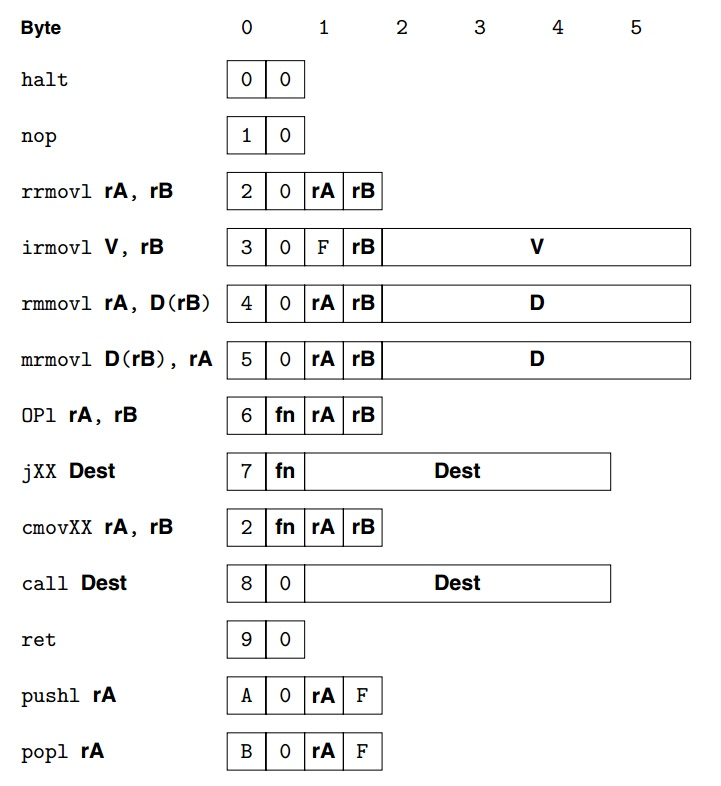
\includegraphics[width=12cm]{instruction.jpg}
	\end{figure}
	\item In the Y86 system, the stack starts at a certain address and grows toward lower addresses, which prevents space conflict.
\end{itemize}
\newpage


\section{Part A}
\subsection{Description}
\begin{itemize}
	\item The program \textbf{sum.ys} was used to sum linked list elements iteratively. We are supposed to add the sum of a list from head to tail using the Y86 codeing rules.
	\item The program \textbf{rsum.ys} is similar to the \textbf{sum.ys}, except it sums linked list elements recursively . We are supposed to add the sum of a list from head to tail using the Y86 codeing rules.
	\item The program \textbf{copy.ys} is used for two purposes. First it copies a block of words from one part of memory to another area of memory. Second it computes the checksum (Xor) of all the words copied.
	
\end{itemize}
\subsection{Solution}
\begin{lstlisting}[language=C,title=sum.ys]
# Initial code
irmovl Stack,%esp
rrmovl %esp,%ebp
irmovl ele1, %edx
#pushl %edx
call sum_list
halt

# Sample linked list
.align 4
ele1:
.long 0x00a
.long ele2
ele2:
.long 0x0b0
.long ele3
ele3:
.long 0xc00
.long 0

sum_list:
pushl %ebp		# Save %ebp
xorl %eax,%eax		# val = 0
rrmovl %esp,%ebp	# Set frame ptr
#pushl %edx
#mrmovl 8(%ebp),%edx	# Get ls
andl %edx,%edx		# ls == 0?
je L4			# Yes, goto done

L5:			# Loop:
mrmovl (%edx),%esi	# t = ls->val
addl %esi,%eax		# val += t
mrmovl 4(%edx),%edx	# ls = ls->next
andl %edx,%edx		# ls == 0?
jne L5			# No, goto done

L4:			# Done:
rrmovl %ebp,%esp	# Restore %esp
popl %ebp		# Restore %ebp
ret			# Return

.pos 0x100
Stack:
\end{lstlisting}
\begin{lstlisting}[language=C,title=rsum.ys]
# Execution begins at address 0	 		
.pos 0
init:		irmovl Stack, %esp
irmovl Stack, %ebp
jmp Main

# Sample linked list			
.align 4
ele1:		.long 0x00a
.long ele2
ele2:		.long 0x0b0
.long ele3
ele3:		.long 0xc00
.long 0

Main: 		irmovl ele1, %edx
pushl %ebp
rrmovl %esp, %ebp
pushl %edx
call rsum_list
rrmovl %ebp, %esp
popl %ebp
halt

# rsum_list - Recursive version of sum_list
# int rsum_list(list_ptr ls)				
rsum_list:	pushl   	%ebp
rrmovl    	%esp,%ebp
mrmovl    	0x8(%ebp),%edx	# ls
xorl    	%eax,%eax	# val=0
pushl   	%ebx		# save %ebx
andl   		%edx,%edx	# ls==0?
je     		End		# if so, gotoEnd
mrmovl    	(%edx),%ebx	# ls->val
mrmovl		0x4(%edx),%ecx	# ls->next
pushl  		%ecx	
# push ls->next as the first parameter
call 		rsum_list	
# call rsum_list by recursion
addl		%ebx,%eax	# val+=ls->val
End:		mrmovl  0xfffffffc(%ebp),%ebx
# restore %ebx
rrmovl 		%ebp, %esp
popl		%ebp
ret

.pos	0x100	
Stack:
\end{lstlisting}
\begin{lstlisting}[language=C,title=copy.ys]
.pos 0
init:	irmovl Stack, %esp
irmovl Stack, %ebp
jmp Main

.align 4
# Source block
src:
.long 0x00a
.long 0x0b0
.long 0xc00
# Destination block
dest:
.long 0x111
.long 0x222
.long 0x333

Main:	irmovl $3,%eax
pushl %eax
irmovl dest,%edx
pushl %edx
irmovl src,%ecx
pushl %ecx
call Copy
halt

Copy:	pushl %ebp
rrmovl %esp,%ebp
mrmovl 8(%ebp),%ecx	#ecx = src
mrmovl 12(%ebp),%ebx	#ebx = dest
mrmovl 16(%ebp),%edx	#edx = len
irmovl $0,%eax		#result = 0
andl %edx,%edx
je End
Loop:	mrmovl (%ecx),%esi	#get *src
rmmovl %esi,(%ebx)	#scr = dest
xorl %esi,%eax		#result ^= src
irmovl $4,%edi		#set %edi to 4
addl %edi,%ecx		#+4
addl %edi,%ebx		#+4
irmovl $-1,%edi	        #set %edi to -1
addl %edi,%edx          #len - 1
jne    Loop             #Stop when 0


End:	popl %ebp
rrmovl %ebp, %esp
popl %ebp
ret

.pos 0x100
Stack:
\end{lstlisting}

\subsection{Analysis}
\subsubsection{sum.ys}
\begin{itemize}
	\item For the program \textbf{sum.ys}, the line $1\sim 19$ and line $42\sim 43$ are the preparatory work and do not need further explanation.
	For the main part, which is the sum.ys, first we store the $\%ebp$ part to stack,  then we set $\%eax$ to zero as the inital sum value, $\%edx$ as the inital list position, then if the list has reached its end, we jump to state L4, which restore the value. If not, we goto the LOOP L5 part.
	\item In the L5 part, first $\%eax+=\%esi$ to add to the sum, then $(\%edx)+4$ to goto the list's next elements. After doing that, again we judge whether the list has reached its end and the condition is exactly the same.
	\item Based the outcome of this program, $\%eax$ stores the overall sum value, which is $0xcba$, $\%ebp$ get popped and get its inital value, which is the $0x100$, $\%esi$ stores the last elements of the list, which is $\%0xc00$, which proves that our program is correct.
\end{itemize}

\subsubsection{rsum.ys}
\begin{itemize}
	\item For the program \textbf{rsum.ys}, the line $1\sim 14$ and line $47\sim 48$ are the preparatory work and do not need further explanation.
	For the main part, first we let $\%edx$ stores the elel, which is the beginning, then we save $\%edx$ and call $rsum\_list$.
	\item For the $rsum\_list$ part(line$27\sim 45$),which is the recursive version of the $sum\_list$, first we use $\%edx$ to get starting adddress, $\%eax$ to get the inital result which is $0$, then we save $\%ebx$ and compare whether $\%edx$ is zero or not. If so, goto $end$, else, goto the next part, which is the recursive part. It is worth noting that in line $39$ the constant number $0xfffffffc$ is $-4$ and we use this operation to restore $\%ebx$, and in line $17$, we push $\%ebp$, in line $44$, we pop $\%ebp$, with these two operations we can get the old version of $\%ebp$ which is key to our recursive part.
	\item Based the outcome of this program, $\%ebp$ pop out and its inital value is $0x100$, $\%eax$ stores the overall sum value $0xcba$, which proves that our program is correct.
\end{itemize}

\subsubsection{copy.ys}
\begin{itemize}
	\item For the program \textbf{copy.ys}, the line $1\sim 16$ and line $51\sim 52$ are the preparatory work and do not need further explanation.
	For the main part(line $18\sim 25$), first we change $\%eax$ to $3$, $\%edx$ to the $dest$, $\%ecx$ to the $src$ and store the value to the stack, then we call Copy function and halt.
	\item For the Copy function(line $28\sim 43$), first we let $\%ebp$ store $\%esp$, $\%ecx$ store $src$, $\%ebx$ store $dest$, $\%edx$ store the length, $\%eax$ stores the inital value of the result which is $0$, then we compare whether the copy function has reached its end, is so, goto the End part, else, goto the Loop part.
	\item For the Loop part, first we get the address of the $scr$, then we begin the copy process, while we add the $src$ and $dest$ by 4 to move to the next address, in the meantime we let $len-1$ to serve as flag to decide when to stop.
	\item Based the outcome of this program, register $\%eax$ do the $xorl$ instruction with each value and then add to $\%eax$, so the last value of $\%eax$ is $0xcba$, also the address $0x0020$ value is changed from $0x111$ to $0xa$, the address $0x0024$ value is changed from $0x222$ to $0xb0$, the address $0x0028$ value is changed from $0x333$ to $0xc00$, which proves that our program is correct.
\end{itemize}

\subsection{Outcome}
\begin{figure}[H]
	\centering
	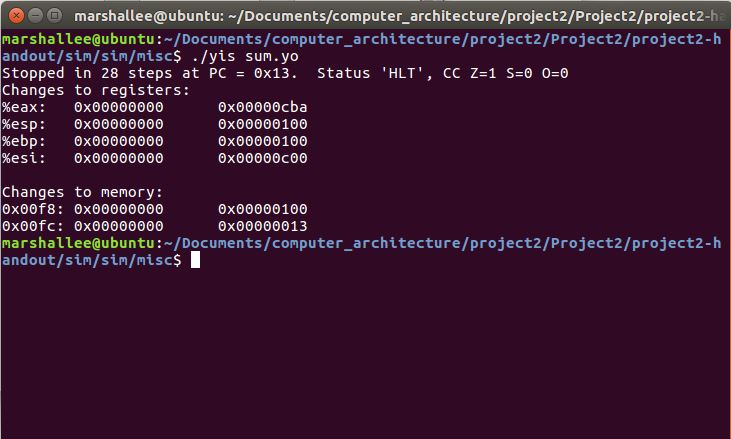
\includegraphics[width=12cm]{sum.jpg}	
\end{figure}



\begin{figure}[H]
	\centering
	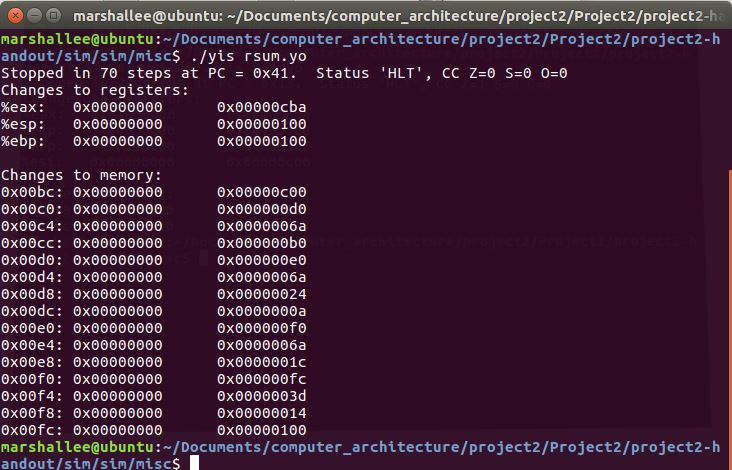
\includegraphics[width=12cm]{rsum.jpg}
\end{figure}
\begin{figure}[H]
	\centering
	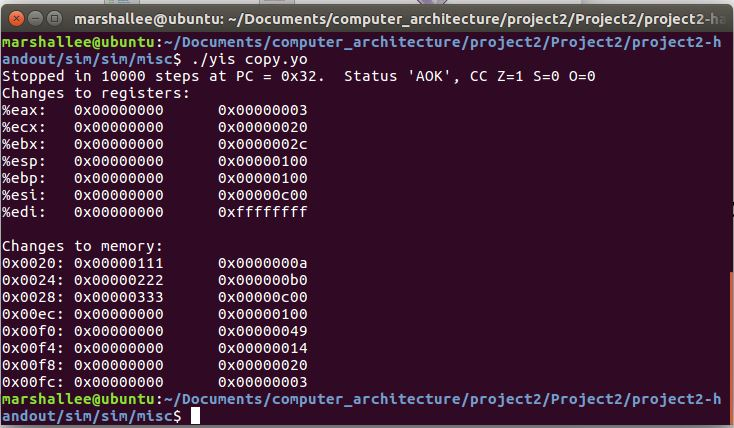
\includegraphics[width=12cm]{copy.jpg}
\end{figure}
\newpage

\section{Part B}		
\subsection{Description}
In this part, we are asked to add a new instruction $iaddl$ to the SEQ processor, this instruction is meant to add a constant to a register.

\subsection{Solution}

\begin{table}[H]
	\centering
	\begin{tabular}{r|p{3in}} \hline
		\hline
		
		
		
		Stage	& iaddl V, rB \\
		\hline
		\hline
		Fetch&  icode:ifun$\leftarrow$$M_1$[PC]\\
		&  rA:rB $\leftarrow$ $M_1$[PC+1]\\
		&  valC$\leftarrow$ $M_4$[PC+2]\\
		&  valP$\leftarrow$ PC+6\\
		\hline
		Decode&   valB$\leftarrow$R[rB]\\
		\hline
		Execute&  valE$\leftarrow$valB $ADD$ valC  \\
		\hline
		Memory&   \\
		\hline
		Write back& R[rB]$\leftarrow$valE  \\
		\hline
		PC update&   PC$\leftarrow$ valP\\
		\hline
	\end{tabular}
\end{table}

Since the code in seq-full.hcl is quite long, I only list the part where we have made changes.
\begin{lstlisting}[language=C++,title=Fetch Stage]
int main(void)
{
	struct sigaction handler;
	handler.sa_handler = handler_SIGINT;
	sigaction(SIGINT, &handler, NULL);
	//strcpy(buffer, "\nCaught Control C\n");

	
	while(1)
	{
		printf("COMMAND->");
		setup(inputBuffer, args, &background);
		if(!strlen(inputBuffer)) continue;
		fpid = fork();
		switch(fpid)
		{
			case -1: perror("fork failed"); exit(1);
			case 0 : execvp(args[0], args); perror("execvp failed"); exit(1);
			default:
				if(background) while(wait(&exitstatus)!= fpid);
		}
		inputBuffer[0] = 0;
	}
	return 0;
}
\end{lstlisting}

\subsection{Analysis}
It can be implemented by first using $irmovl$ instruction to let the register contains the constant number, then we can use $addl$ instruction to add the constant number to the destination register. Since there are roughly four stages in the Y86 instruction set, we will fully discuss this part reagarding each stages.
\begin{itemize}
	\item For the Fetch Stage, first we should add the $IIADDL$ instruction to the $instr\_valid$, then we should add the $IIADDL$ instruction to the $need\_regids$ set, indicating that we should register to do this operation. Finally since we need a constant to do the addition, we need to add the $IIADDL$ instruction to the $need\_valc$ set.
	\item For the Decode Stage, first we need to add the $IIADDL$ instruction to the $srcB$ set, indicating that we put the register value of $rB$ in this part, then we need to add the $IIADDL$ instruction to the $dstE$ set, indicating that we store the value in the destination E, which is to the same register of $rB$.
	\item For the Execute Stage, first we should add the $IIADDL$ instruction to the $aluA$ part, indicating that the ALU operation need the $valC$, which is the constant value, then we should add the $IIADDL$ instruction to the $aluB$ part, indicating that the ALU operation need the $valB$, finally we should add the $IIADDL$ instruction to the $set\_cc$ part, indicating that this instruction may lead the flag register to change.
	\item For the Memory Stage, since this instruction is to add a constant number to a register, so the Memory Stage don't have to change.
\end{itemize}

\subsection{Outcome}
\begin{figure}[H]
	\centering
	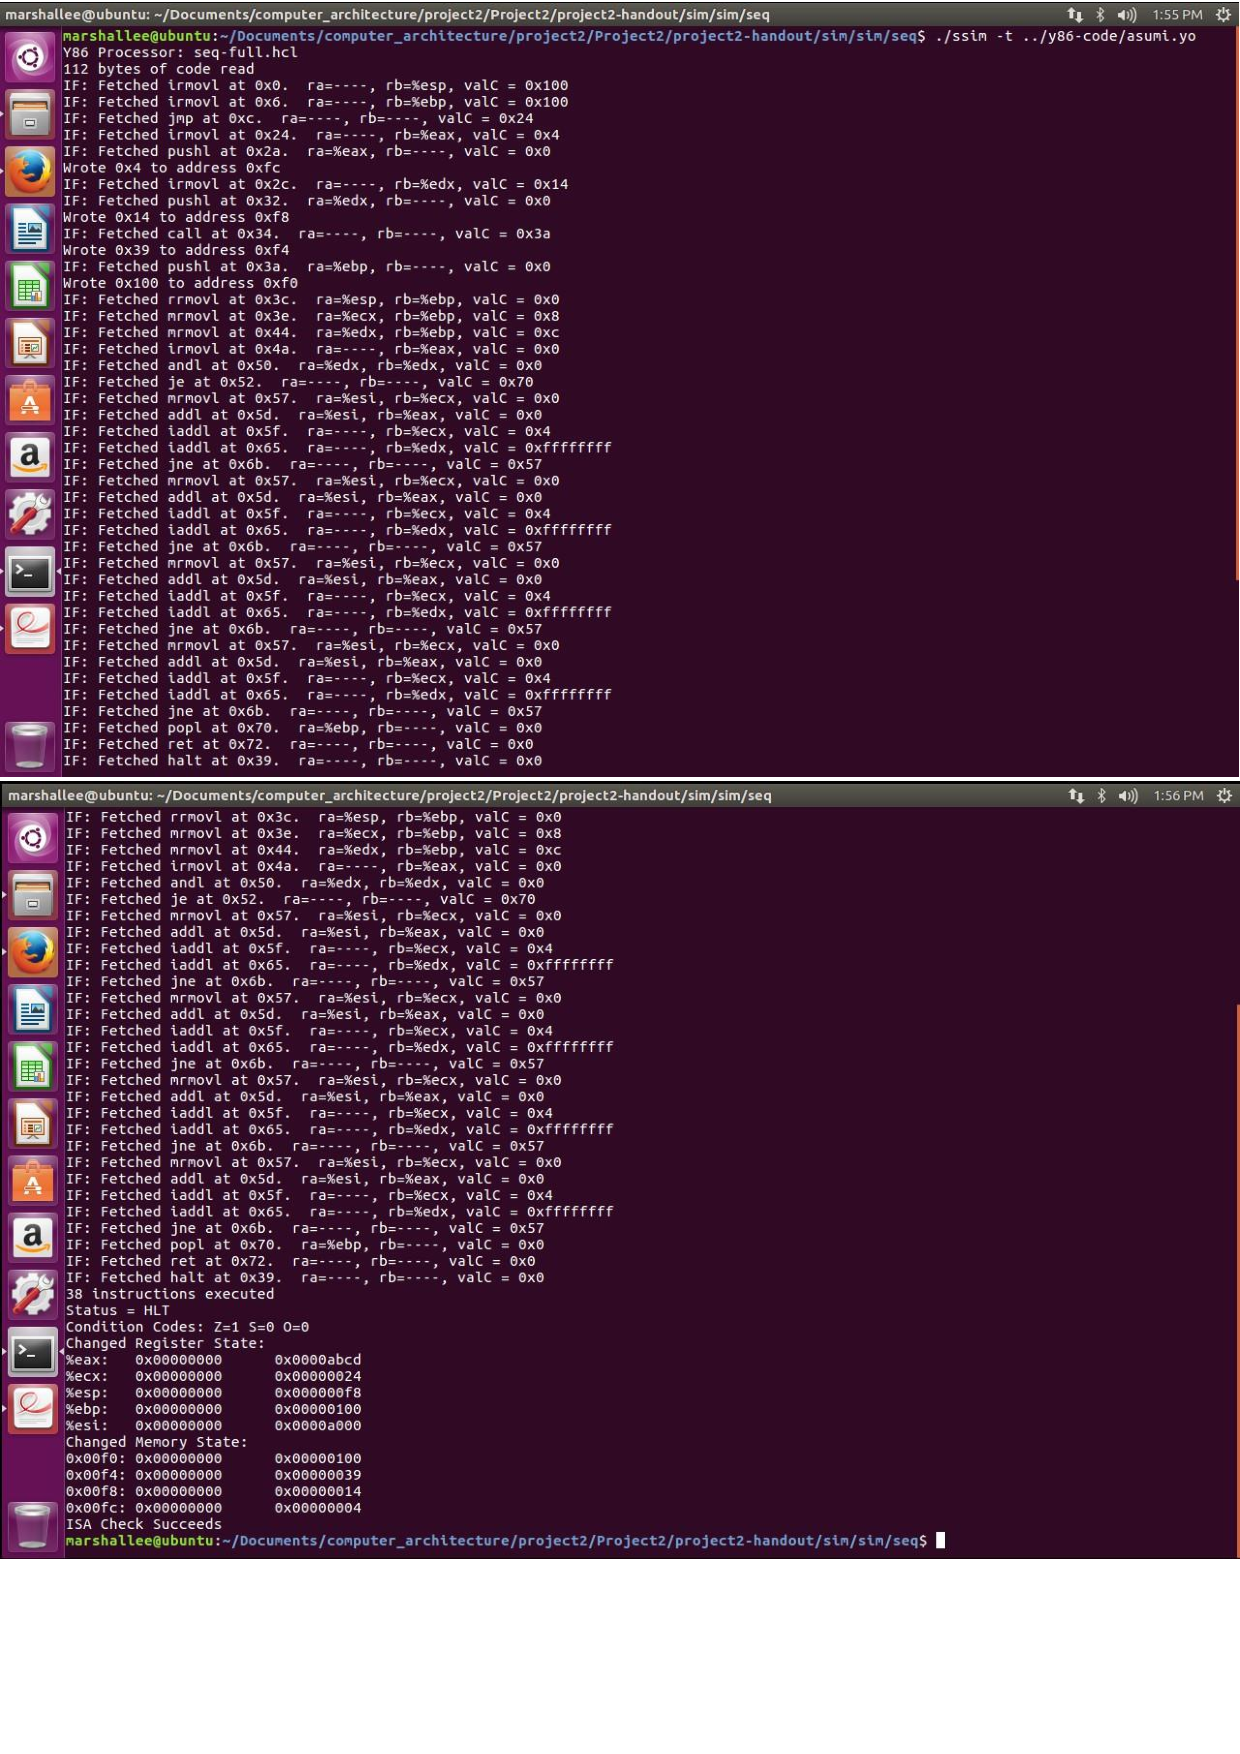
\includegraphics[width=12cm]{iaddl.pdf}
\end{figure}
\newpage

\section{Part C}		
\subsection{Description}
\begin{itemize}
	\item The program \textbf{ncopy.ys} copies a len-element integer array $src$ to a non-overlapping $dst$, returning the count number of positive integers contained in $src$.
	\item In this part, we need to minimize the running time of \textbf{ncopy.ys} as less as possible. We use 3 ways to decrease running time: decrease jump instruction, use iaddl instruction and decrease hazards.
	\item As we have learned in the class, the $jump$ instructions (including $jmp$, $jle$, $jl$, $je$, $jne$, $jge$ and $jg$ in Y86 instructions). Of course we can write one loop to solve this problem, but it costs to much time. So we use some other methods to solve this problem.
	\item In traditional add instruction, we can only store the instant number in registers and add the values in registers, which increase the running time. The iaddl instruction can do the add instruction between instant number and register, which decrease the running time.
	\item If we store a value in a register and the next instruction is to use the value in this register, there must be staff. So we use 2 registers to do it so to decrease staffs, which also decrease our running time.
\end{itemize}

\subsection{Solution}
\begin{lstlisting}[language=C++,title=ncopy.ys]
#/* $begin ncopy-ys */
#######################################
# ncopy.ys - Copy a src block of len ints to dst.
# Return the number of positive ints (>0) contained in src.
#
# Include your name and ID here.
#
# Describe how and why you modified the baseline code.
#
#######################################
# Do not modify this portion
# Function prologue.
ncopy:	pushl %ebp		# Save old frame pointer
rrmovl %esp,%ebp	# Set up new frame pointer
pushl %esi		# Save callee-save regs
pushl %ebx
pushl %edi
mrmovl 8(%ebp),%ebx	# src
mrmovl 16(%ebp),%edx	# len
mrmovl 12(%ebp),%ecx	# dst
#######################################
xorl  %eax, %eax	# initialize the count to 0

#######################################
Loop8:
iaddl $-8,  %edx	# len = len - 8
andl  %edx, %edx	# to see if the len is less than 0
jl Loop4

mrmovl (%ebx), %esi
mrmovl 4(%ebx), %edi
rmmovl %esi, (%ecx)
andl %esi, %esi
jle StageOneOf8
iaddl $1, %eax

StageOneOf8:
rmmovl %edi, 4(%ecx)
andl %edi, %edi
jle StageTwoOf8
iaddl $1, %eax

StageTwoOf8:
mrmovl 8(%ebx), %esi
mrmovl 12(%ebx), %edi
rmmovl %esi, 8(%ecx)
andl %esi, %esi
jle StageThreeOf8
iaddl $1, %eax

StageThreeOf8:
rmmovl %edi, 12(%ecx)
andl %edi, %edi
jle StageFourOf8
iaddl $1, %eax

StageFourOf8:
mrmovl 16(%ebx), %esi
mrmovl 20(%ebx), %edi
rmmovl %esi, 16(%ecx)
andl %esi, %esi
jle StageFiveOf8
iaddl $1, %eax

StageFiveOf8:
rmmovl %edi, 20(%ecx)
andl %edi, %edi
jle StageSixOf8
iaddl $1, %eax

StageSixOf8:
mrmovl 24(%ebx), %esi
mrmovl 28(%ebx), %edi
rmmovl %esi, 24(%ecx)
andl %esi, %esi
jle StageSevenOf8
iaddl $1, %eax

StageSevenOf8:
rmmovl %edi, 28(%ecx)
andl %edi, %edi
jle Forward8
iaddl $1, %eax

Forward8:
iaddl $32, %ebx
iaddl $32, %ecx
jmp Loop8

#######################################
Loop4:
iaddl $8, %edx
iaddl $-4, %edx
andl  %edx, %edx
jl Loop2

mrmovl (%ebx), %esi
mrmovl 4(%ebx), %edi
rmmovl %esi, (%ecx)
andl %esi, %esi
jle StageOneOf4
iaddl $1, %eax

StageOneOf4:
rmmovl %edi, 4(%ecx)
andl %edi, %edi
jle StageTwoOf4
iaddl $1, %eax

StageTwoOf4:
mrmovl 8(%ebx), %esi
mrmovl 12(%ebx), %edi
rmmovl %esi, 8(%ecx)
andl %esi, %esi
jle StageThreeOf4
iaddl $1, %eax

StageThreeOf4:
rmmovl %edi, 12(%ecx)
andl %edi, %edi
jle Forward4
iaddl $1, %eax

Forward4:
iaddl $16, %ebx
iaddl $16, %ecx
iaddl $-4, %edx
jmp Loop2

#######################################
Loop2:
iaddl $4, %edx
iaddl $-2, %edx
andl %edx, %edx
jl Loop1

mrmovl (%ebx), %esi
mrmovl 4(%ebx), %edi
rmmovl %esi, (%ecx)
andl %esi, %esi
jle StageOneOf2
iaddl $1, %eax

StageOneOf2:
rmmovl %edi, 4(%ecx)
andl %edi, %edi
jle Forward2
iaddl $1, %eax

Forward2:
iaddl $8, %ebx
iaddl $8, %ecx
iaddl $-2, %edx
jmp Loop1

#######################################
Loop1:
iaddl $2, %edx
iaddl $-1, %edx
andl %edx, %edx
jl Done

mrmovl (%ebx), %esi
rmmovl %esi, (%ecx)
andl %esi, %esi
jle Done
iaddl $1, %eax
jmp Done
#######################################
# Do not modify the following section of code
# Function epilogue.
Done:
popl %edi               # Restore callee-save registers
popl %ebx
popl %esi
rrmovl %ebp, %esp
popl %ebp
ret
#######################################
# Keep the following label at the end of your function
End:
#/* $end ncopy-ys */
\end{lstlisting}


\begin{lstlisting}[language=C++,title=Fetch Stage]
# Is instruction valid?
bool instr_valid = f_icode in
{ INOP, IHALT, IRRMOVL, IIRMOVL, IRMMOVL, IMRMOVL,
IOPL, IJXX, ICALL, IRET, IPUSHL, IPOPL, IIADDL};

# Does fetched instruction require a regid byte?
bool need_regids =
f_icode in { IRRMOVL, IOPL, IPUSHL, IPOPL,
IIRMOVL, IRMMOVL, IMRMOVL, IIADDL};

# Does fetched instruction require a constant word?
bool need_valC =
f_icode in { IIRMOVL, IRMMOVL, IMRMOVL, IJXX, ICALL, IIADDL};
\end{lstlisting}
\begin{lstlisting}[language=C,title=Decode Stage]
## What register should be used as the B source?
int d_srcB = [
D_icode in { IOPL, IRMMOVL, IMRMOVL, IIADDL } : D_rB;
D_icode in { IPUSHL, IPOPL, ICALL, IRET } : RESP;
1 : RNONE;  # Don't need register
];

## What register should be used as the E destination?
int d_dstE = [
D_icode in { IRRMOVL, IIRMOVL, IOPL, IIADDL} : D_rB;
D_icode in { IPUSHL, IPOPL, ICALL, IRET } : RESP;
1 : RNONE;  # Don't write any register
];
\end{lstlisting}
\begin{lstlisting}[language=C,title=Execute Stage]
## Select input A to ALU
int aluA = [
E_icode in { IRRMOVL, IOPL } : E_valA;
E_icode in { IIRMOVL, IRMMOVL, IMRMOVL, IIADDL} : E_valC;
E_icode in { ICALL, IPUSHL } : -4;
E_icode in { IRET, IPOPL } : 4;
# Other instructions don't need ALU
];

## Select input B to ALU
int aluB = [
E_icode in { IRMMOVL, IMRMOVL, IOPL, ICALL,
IPUSHL, IRET, IPOPL, IIADDL} : E_valB;
E_icode in { IRRMOVL, IIRMOVL } : 0;
# Other instructions don't need ALU
];

## Should the condition codes be updated?
bool set_cc = E_icode in {IOPL , IIADDL} ;
\end{lstlisting}


\subsection{Analysis}
\subsubsection{ncopy.ys}
\begin{figure}[H]
	\centering
	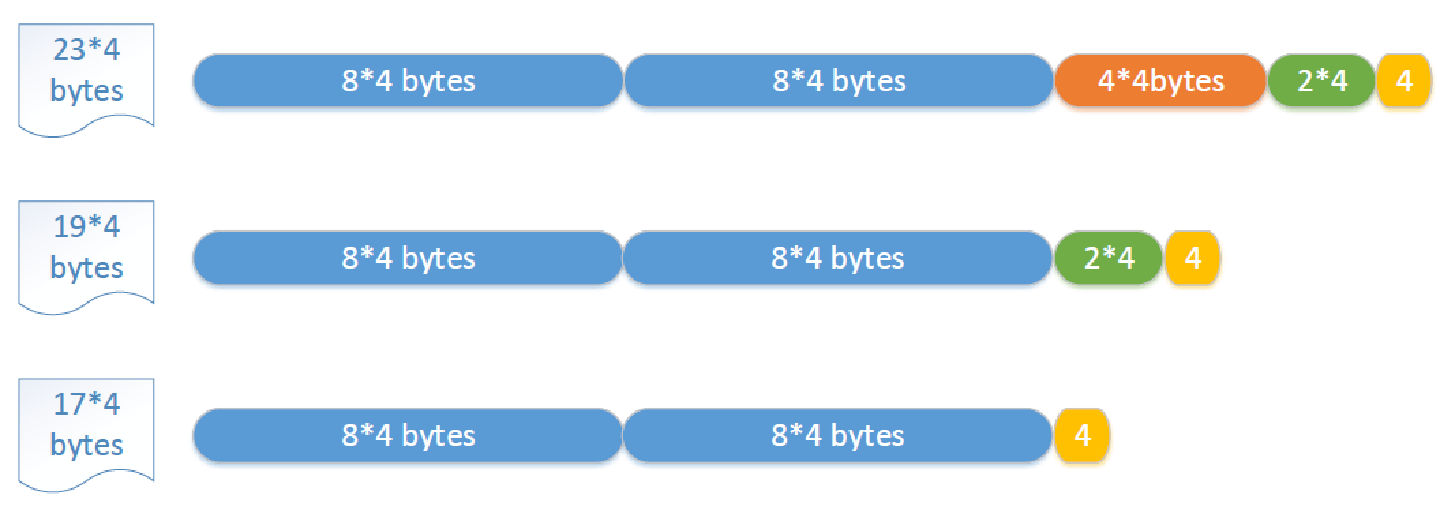
\includegraphics[width=12cm]{Gantt.pdf}
\end{figure}
\begin{itemize}
	\item We use 3 ways to decrease running time: decrease jump instruction, use iaddl instruction and decrease hazards. To explain our solution clearly, we provide the above picture to express the overview of our solution.
	\item Our main idea is: In each copy instruction, we copy $4\ bytes$. Firstly, we copy each $8*4\ bytes$ in a loop until the left data needed to copy is less than $8*4\ bytes$. Secondly, we check if the left data is more or equal to $4*4\ bytes$. If so, we copy $4*4\ bytes$ in this step. Thirdly, we check if the left data is more or equal to $2*4\ bytes$. If so, we copy $2*4\ bytes$ in this step. Finally, we check if there are still $1*4\ bytes$ left. If so, we copy these $4\ bytes$ and end the problem. Since we need to return the count number of positive integers contained in $src$, we will do a judge after each copy instruction to decided if we need to increase the count by 1.
	\item For the instruction iaddl, we will explain why we use it. In traditional instructions, if we want to add an instant number and a value in register, we need to store this number in a register and add values in 2 registers, which need 2 instruction to do this. However, the iaddl instruction allow us to add an instant number and a value in register in just 1 instruction. This will decrease the running time.
	\item For the registers, we define $esi$ and $edi$ to store the value of contiguous 2 words(4 bytes each word). We define $ebx$ to store the address of current $src$ and $dst$ to store the address of current $dst$. We define $edx$ to store the $len$ of left words needed to copy. We define $eax$ to store the count of positive integers in our copyed data.
	\item For register $esi$ and $edi$, we will explain why we use 2 register to store the copy integers. Assume we just use one register, such as $esi$ to do this job. Since the next instruction is to copy the value of $esi$ to $ecx$, there must be staff. However, if we use 2 registers, there are 1 instruction using $edi$ between these 2 instructions using $esi$, there will be no staff. This method can decrease the running time.
	\item For the Loops, we define 4 main blocks: $Loop8$, $Loop4$, $Loop2$ and $Loop1$. However, only the $Loop8$ is the "real" Loop which means only $Loop8$ can be excuted more than 1 time. In the above picture, blue means $Loop8$, oringe means $Loop4$, green means $Loop2$ and yellow means $Loop1$. We provide following picture to represent the relations among these Loop.
	\begin{figure}[H]
		\centering
		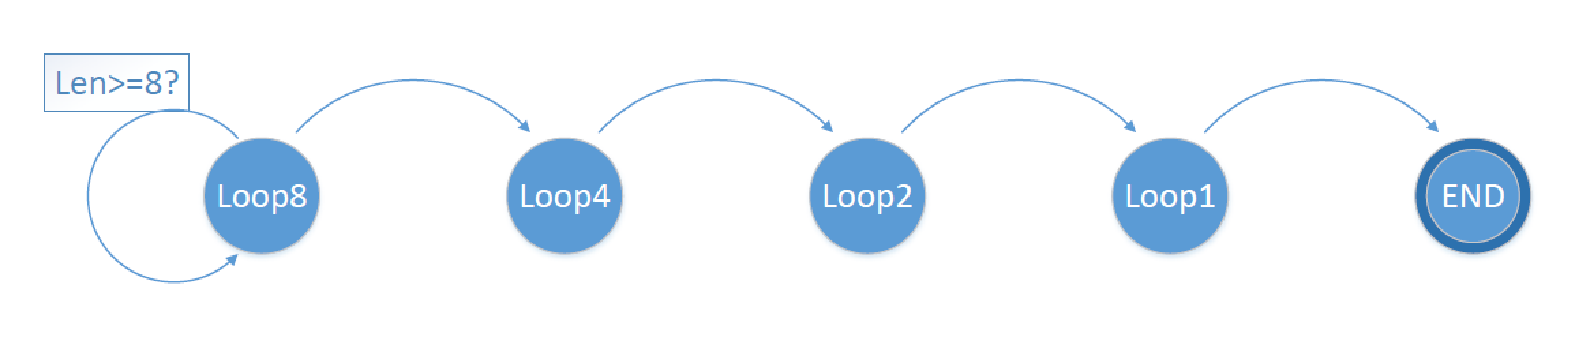
\includegraphics[width=12cm]{Spot.pdf}
	\end{figure}
	\item We take $Loop4$ for example. First we plus 4 to $edx$ and check if it is less than 0. If it is, the program will jump to $Loop2$. Else, we do 4 copy instructions in $Loop4$. The register $esi$ and $edi$ stores the current data we need to copy. After each copy instruction, we will check if the data is a positive integer. If it is, the register $eax$ will be added by 1. Else, the problem will ignore the add instruction and jump to next copy instruction.
	\item Assume we need to copy $n$ words and n is a very large number. Assume the count number of positive integers contained in $src$ is $m$. In our progress, we need $O(log_{8}^n+m)$ jumps. That explains why we use this loop method to decrease the number of jump. Since if we just use 1 loop to do this job, we need $O(n)$ jumps.
\end{itemize}
\subsubsection{pipe-full.hcl}
The analysis in "pipe-full.hcl" is very similar to part B.
\begin{table}[!h]
	\centering
	\begin{tabular}{r|p{3in}} \hline
		\hline
		
		
		
		Stage	& iaddl V, rB \\
		\hline
		\hline
		Fetch&  icode:ifun$\leftarrow$$M_1$[PC]\\
		&  rA:rB $\leftarrow$ $M_1$[PC+1]\\
		&  valC$\leftarrow$ $M_4$[PC+2]\\
		&  valP$\leftarrow$ PC+6\\
		\hline
		Decode&   valB$\leftarrow$R[rB]\\
		\hline
		Execute&  valE$\leftarrow$valB $ADD$ valC  \\
		\hline
		Memory&   \\
		\hline
		Write back& R[rB]$\leftarrow$valE  \\
		\hline
		PC update&   PC$\leftarrow$ valP\\
		\hline
	\end{tabular}
\end{table}
\begin{itemize}
	\item For the Fetch Stage, first we should add the $IIADDL$ instruction to the $instr\_valid$, then we should add the $IIADDL$ instruction to the $need\_regids$ set, indicating that we need register to do this operation. Finally since we need a constant to do the addition, we need to add the $IIADDL$ instruction to the $need\_valC$ set.
	\item For the Decode Stage, first we need to add the $IIADDL$ instruction to the $d\_srcB$ set, indicating that we put the register value of $rB$ in this part, then we need to add the $IIADDL$ instruction to the $d\_dstE$ set, indicating that we store the value in the destination E, which is to the same register of $rB$.
	\item For the Execute Stage, first we should add the $IIADDL$ instruction to the $aluA$ part, indicating that the ALU operation need the $valC$, which is the constant value, then we should add the $IIADDL$ instruction to the $aluB$ part, indicating that the ALU operation need the $valB$, finally we should add the $IIADDL$ instruction to the $set\_cc$ part, indicating that this instruction may lead the flag register to change.
	\item For the Memory Stage, since this instruction is to add a constant number to a register, so the Memory Stage don't have to change.
\end{itemize}

\subsection{Outcome}
\begin{figure}[H]
	\centering
	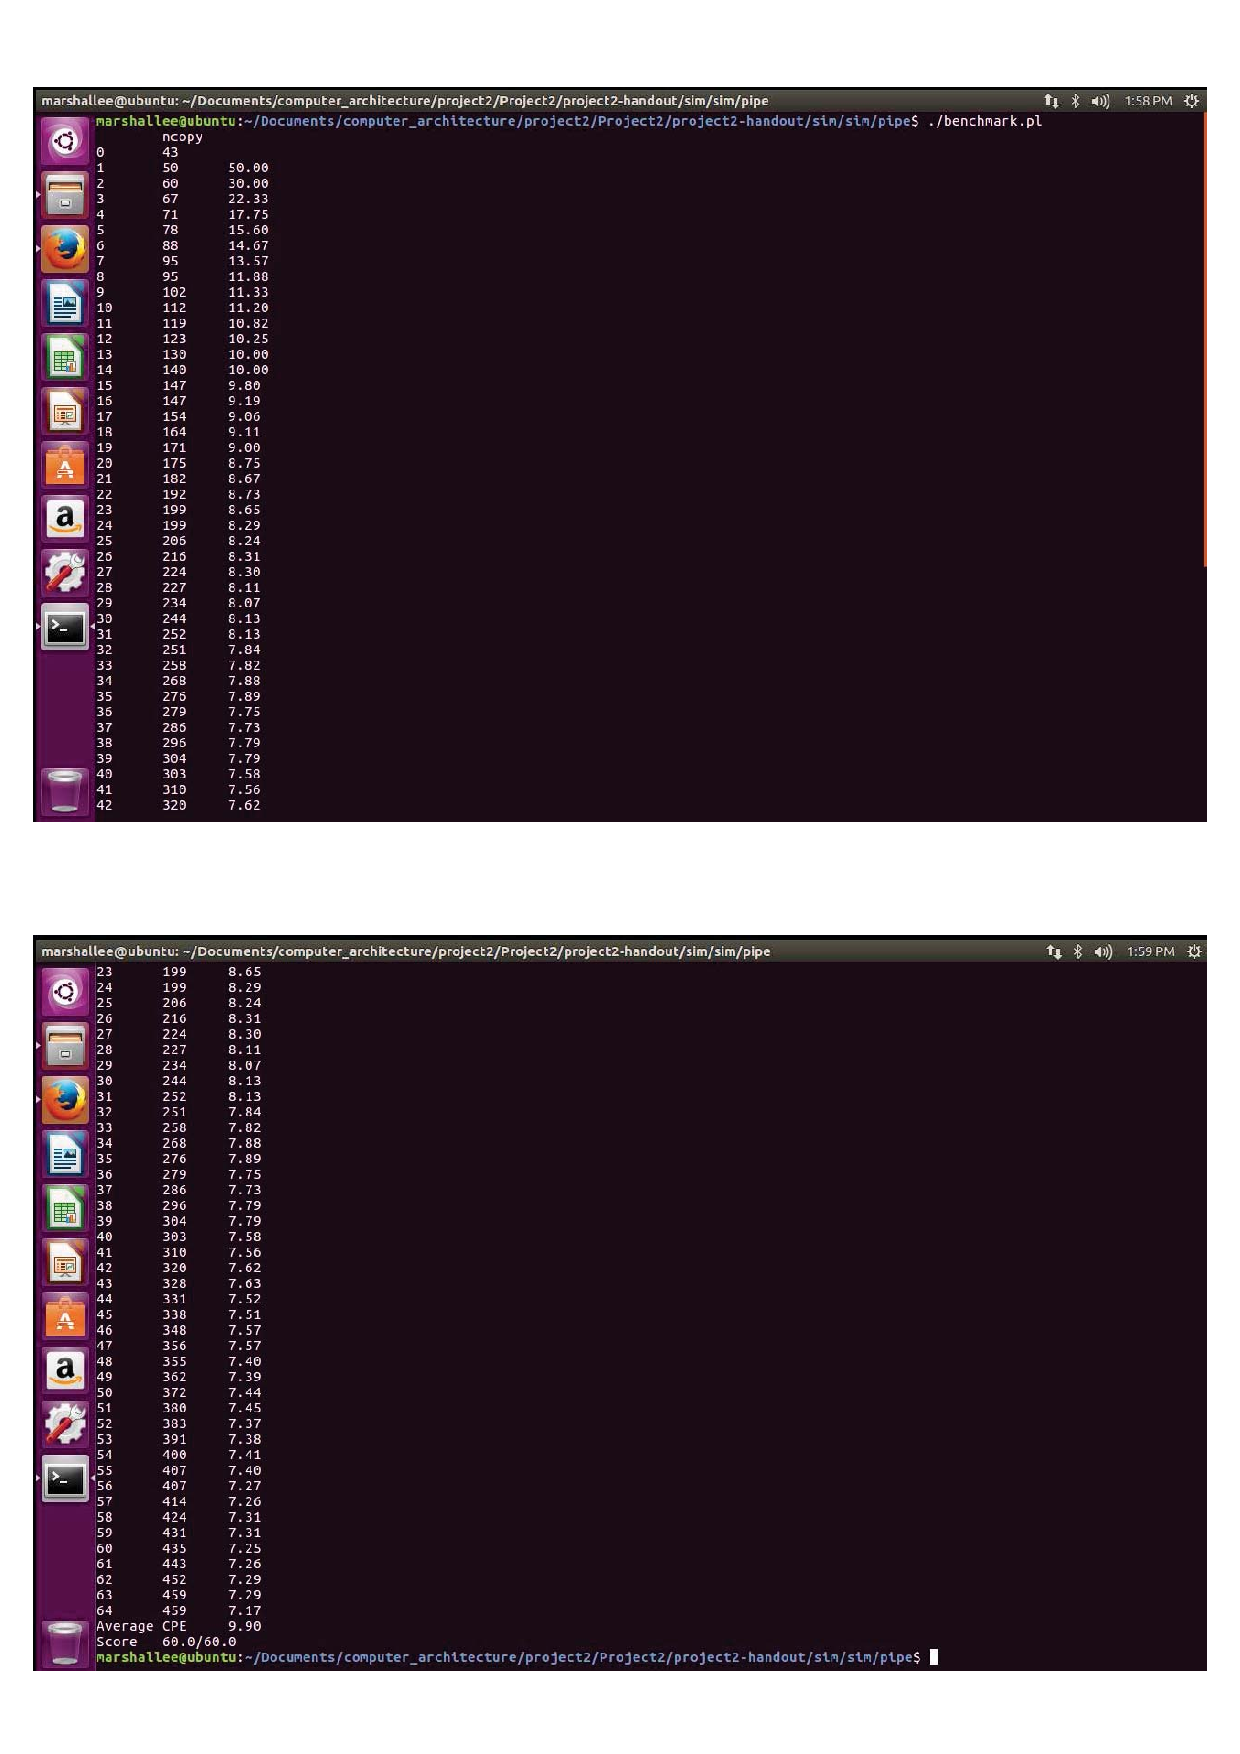
\includegraphics[width=12cm]{ncopy_benchamrk.pdf}
\end{figure}
\begin{figure}[H]
	\centering
	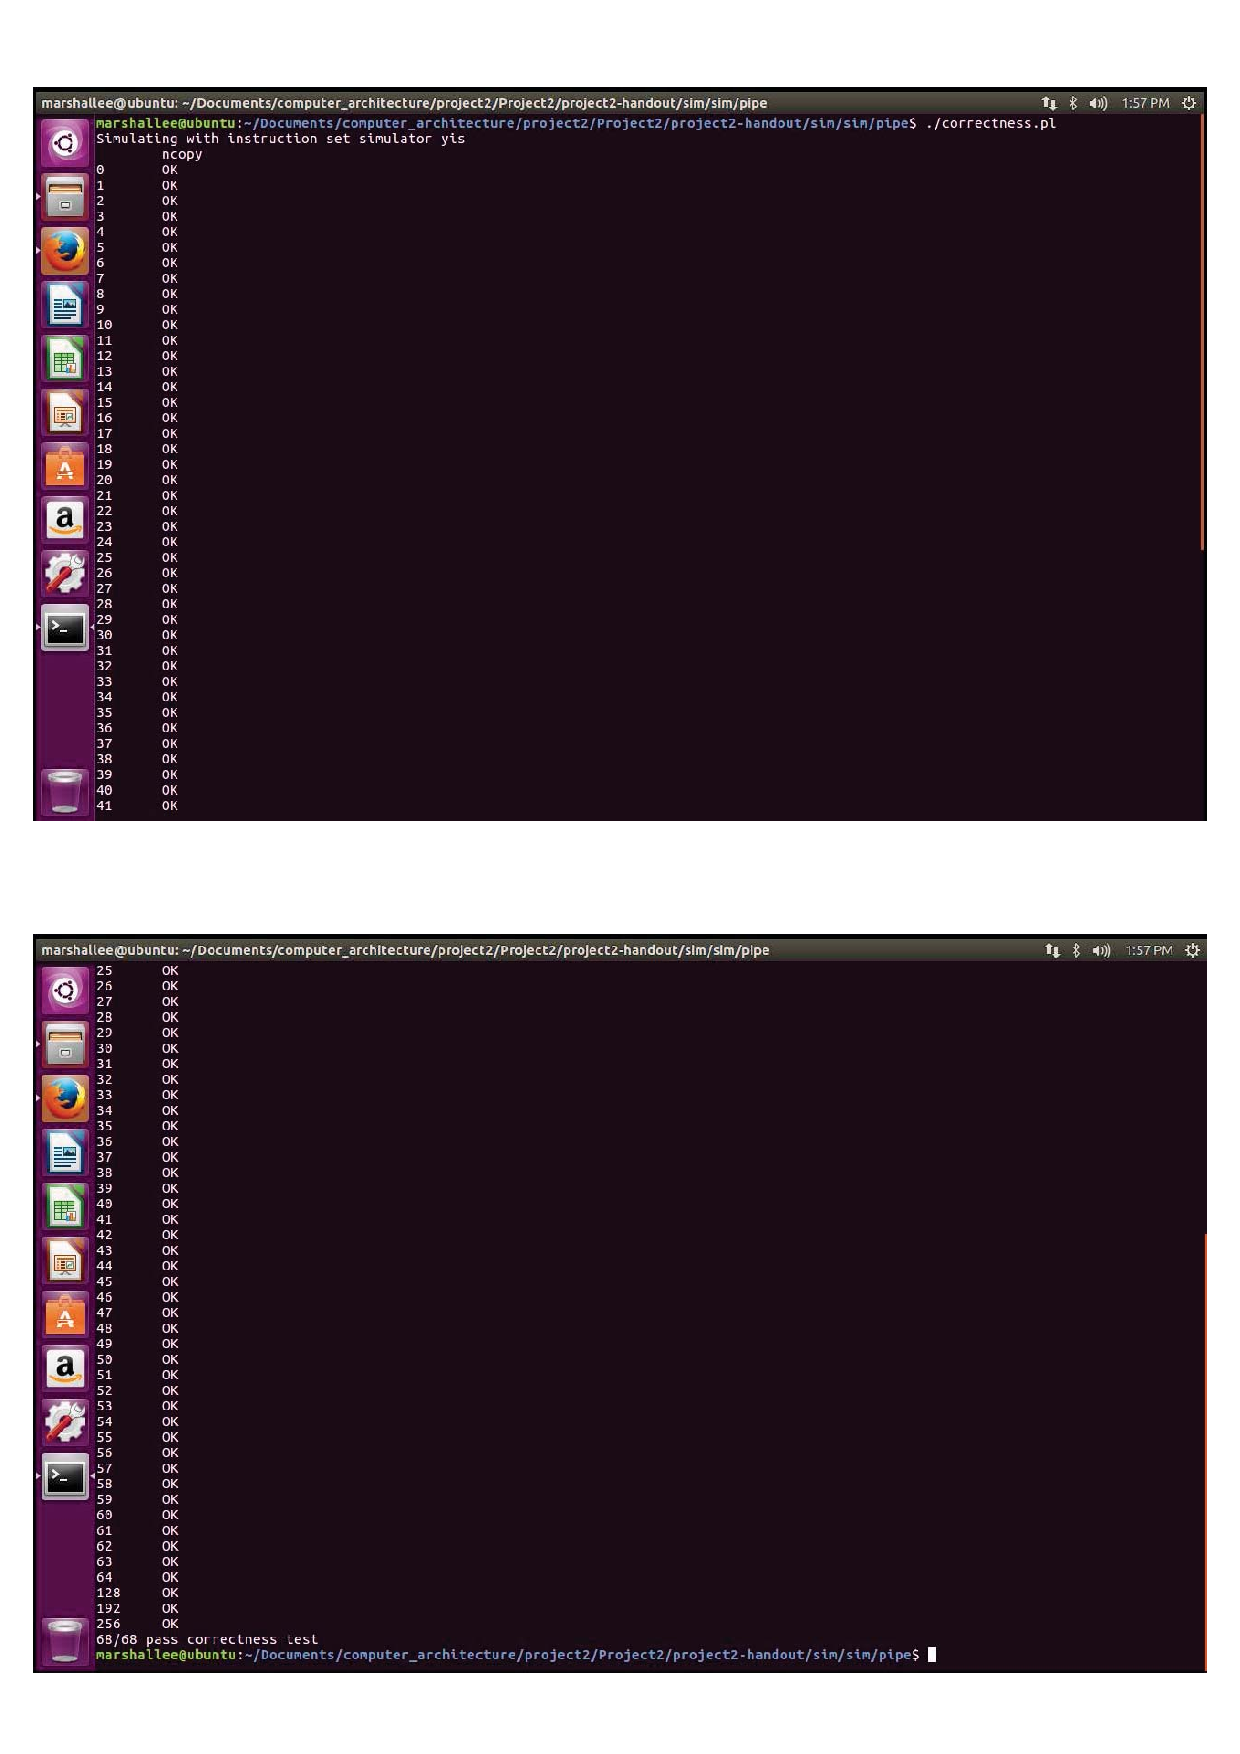
\includegraphics[width=12cm]{ncopy_correctness.pdf}
\end{figure}

\section{Task Assignments}

Li Minchao write codes for partA, partB and partC.

Wang Chenyang write description and report for partC and integrate the report.

Qiang Zhiwen write description and report for partA and partB and write preknowledge of report.
\end{document}
